\documentclass[aspectratio=169]{../latex_main/tntbeamer}  % you can pass all options of the beamer class, e.g., 'handout' or 'aspectratio=43'
\usepackage{dsfont}
\usepackage{bm}
\usepackage[english]{babel}
\usepackage[T1]{fontenc}
%\usepackage[utf8]{inputenc}
\usepackage{graphicx}
\graphicspath{ {./figures/} }
\usepackage{algorithm}
\usepackage[ruled,vlined,algo2e,linesnumbered]{algorithm2e}
\usepackage{hyperref}
\usepackage{booktabs}
\usepackage{mathtools}

\usepackage{amsmath,amssymb}

\DeclareMathOperator*{\argmax}{arg\,max}
\DeclareMathOperator*{\argmin}{arg\,min}

\usepackage{amsbsy}
\newcommand{\vect}[1]{\bm{#1}}
%\newcommand{\vect}[1]{\boldsymbol{#1}}

\usepackage{pgfplots}
\pgfplotsset{compat=1.16}
\usepackage{tikz}
\usetikzlibrary{trees} 
\usetikzlibrary{shapes.geometric}
\usetikzlibrary{positioning,shapes,shadows,arrows,calc,mindmap}
\usetikzlibrary{positioning,fadings,through}
\usetikzlibrary{decorations.pathreplacing}
\usetikzlibrary{intersections}
\pgfdeclarelayer{background}
\pgfdeclarelayer{foreground}
\pgfsetlayers{background,main,foreground}
\tikzstyle{activity}=[rectangle, draw=black, rounded corners, text centered, text width=8em]
\tikzstyle{data}=[rectangle, draw=black, text centered, text width=8em]
\tikzstyle{myarrow}=[->, thick, draw=black]

% Define the layers to draw the diagram
\pgfdeclarelayer{background}
\pgfdeclarelayer{foreground}
\pgfsetlayers{background,main,foreground}

% Requires XeLaTeX or LuaLaTeX
%\usepackage{unicode-math}

\usepackage{fontspec}
%\setsansfont{Arial}
\setsansfont{RotisSansSerifStd}[ 
Path=../latex_main/fonts/,
Extension = .otf,
UprightFont = *-Regular,  % or *-Light
BoldFont = *-ExtraBold,  % or *-Bold
ItalicFont = *-Italic
]
\setmonofont{Cascadia Mono}[
Scale=0.8
]

% scale factor adapted; mathrm font added (Benjamin Spitschan @TNT, 2021-06-01)
%\setmathfont[Scale=1.05]{Libertinus Math}
%\setmathrm[Scale=1.05]{Libertinus Math}

% other available math fonts are (not exhaustive)
% Latin Modern Math
% XITS Math
% Libertinus Math
% Asana Math
% Fira Math
% TeX Gyre Pagella Math
% TeX Gyre Bonum Math
% TeX Gyre Schola Math
% TeX Gyre Termes Math

% Literature References
\newcommand{\lit}[2]{\href{#2}{\footnotesize\color{black!60}[#1]}}

%%% Beamer Customization
%----------------------------------------------------------------------
% (Don't) Show sections in frame header. Options: 'sections', 'sections light', empty
\setbeamertemplate{headline}{empty}

% Add header logo for normal frames
\setheaderimage{
	% 
\includegraphics[height=\logoheight]{figures/TNT_darkv4.pdf}
	
\includegraphics[height=\logoheight]{../latex_main/figures/luh_logo_rgb_0_80_155.pdf}
	% 
\includegraphics[height=\logoheight]{figures/logo_tntluh.pdf}
}

% Header logo for title page
\settitleheaderimage{
	% 
\includegraphics[height=\logoheight]{figures/TNT_darkv4.pdf}
	
\includegraphics[height=\logoheight]{../latex_main/figures/luh_logo_rgb_0_80_155.pdf}
	% 
\includegraphics[height=\logoheight]{figures/logo_tntluh.pdf}
}

% Title page: tntdefault 
\setbeamertemplate{title page}[tntdefault]  % or luhstyle
% Add optional title image here
%\addtitlepageimagedefault{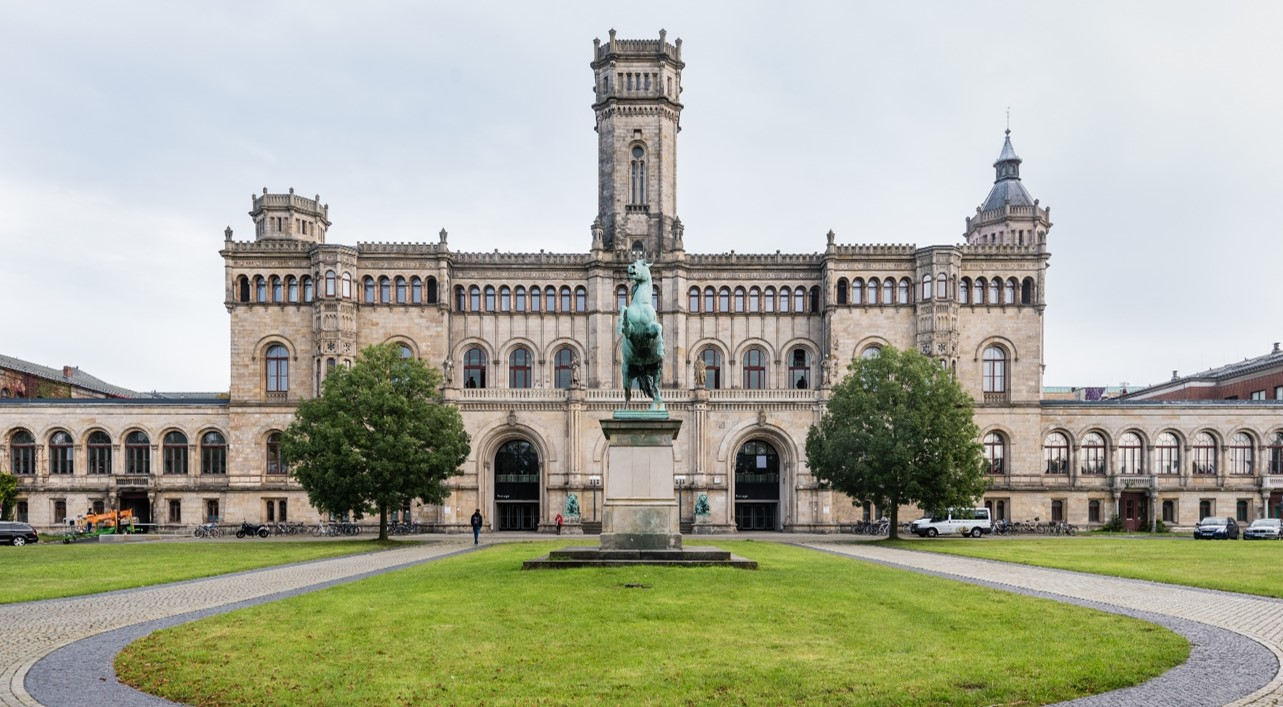
\includegraphics[width=0.65\textwidth]{figures/luh_default_presentation_title_image.jpg}}

% Title page: luhstyle
% \setbeamertemplate{title page}[luhstyle]
% % Add optional title image here
% \addtitlepageimage{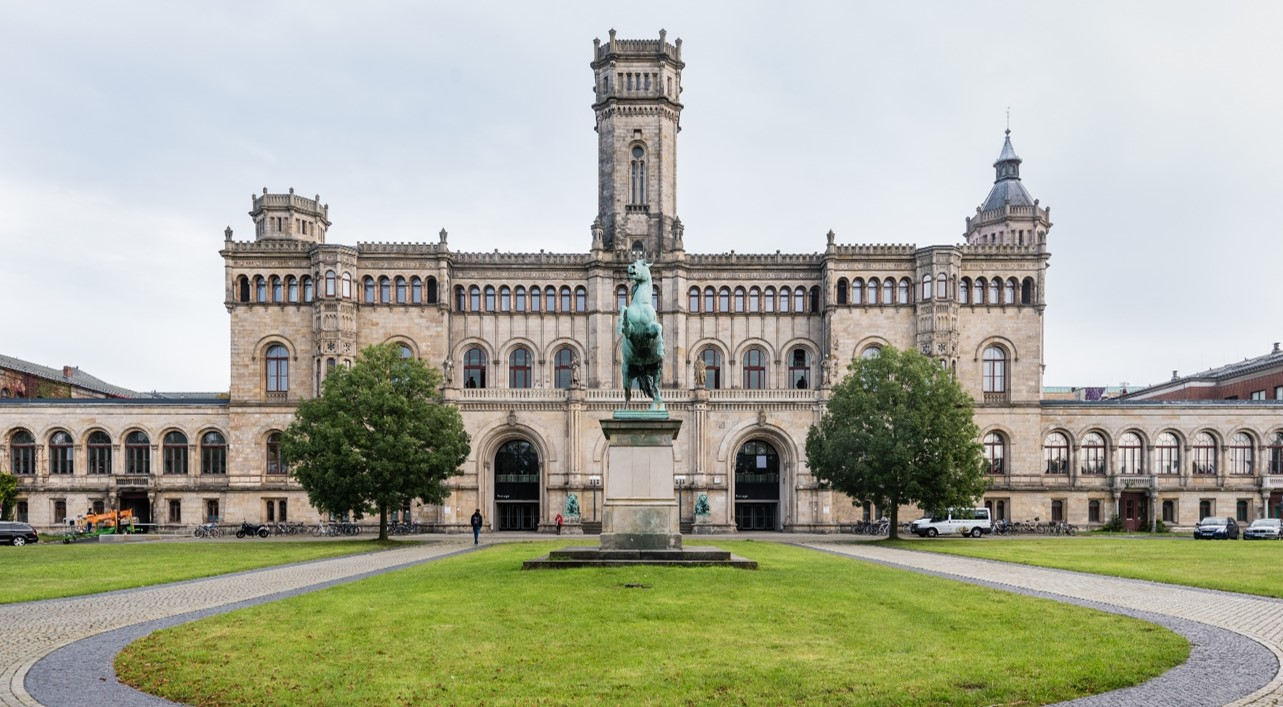
\includegraphics[width=0.75\textwidth]{figures/luh_default_presentation_title_image.jpg}}

\author[Abedjan \& Lindauer]{Ziawasch Abedjan \& Marius Lindauer\\[1em]
	
\includegraphics[height=\logoheight]{../latex_main/figures/luh_logo_rgb_0_80_155.pdf}\qquad
	
\includegraphics[height=\logoheight]{../latex_main/figures/DBIS_Kurzlogo.png}\qquad

\includegraphics[height=\logoheight]{../latex_main/figures/TNT_darkv4}\qquad

\includegraphics[height=\logoheight]{../latex_main/figures/L3S.jpg}	}
\date{Summer Term 2022; \hspace{0.5em} {
\includegraphics[height=1.5em]{../latex_main/figures/Cc-by-nc-sa_icon.svg.png}}; based on \href{https://ds100.org/fa21/}{[DS100]}
}


%%% Custom Packages
%----------------------------------------------------------------------
% Create dummy content
\usepackage{blindtext}

% Adds a frame with the current page layout. Just call \layout inside of a frame.
\usepackage{layout}


%%% Macros
%\renewcommand{\vec}[1]{\mathbf{#1}}
% \usepackage{bm}
%\let\vecb\bm

\title[Introduction]{DS: Gradient Descent}
\subtitle{Gradient Descent in 2D}

\graphicspath{ {./figure/} }
%\institute{}


\begin{document}
	
	\maketitle
	\begin{frame}[c]{Loss Minimization Game}
	    From Fall 2018:
	    \begin{itemize}
	        \item \url{https://tinyurl.com/3dloss18}
	        \item Try playing until you get the “You Win!” message.
	    \end{itemize}
	\end{frame}
	
	
	\begin{frame}{Optimization Goal}
	    Now suppose we change our model so that it has two parameters $\theta_0$ and $\theta_1$.
	    \begin{itemize}
	        \item $\theta_0$ is the y-intercept, and $\theta_1$   is the slope.
	    \end{itemize}
	    \begin{columns}
	        \begin{column}{.5\textwidth}
	                \begin{align*}
	                     &\text{tip} = \hat{\theta}_0 + \hat{\theta}_1 \text{bill}\\
	                     &\Vec{\hat{y}}  = f_{\Vec{\hat{\theta}}}(\mathbb{X}) = \mathbb{X}\Vec{\hat{\theta}}\\
	                     &\mathbb{X} = \left[\begin{array}{cc}
	                                 1 & 16.99 \\
	                                 1 & 10.34 \\
	                                 1 & 21.01 \\
	                                 1 & 23.68 \\
	                                 \vdots & \vdots
	                        \end{array}\right]
	                 \end{align*}
	        \end{column}
	        
	        
	        \begin{column}{.5\textwidth}
	                \\
	                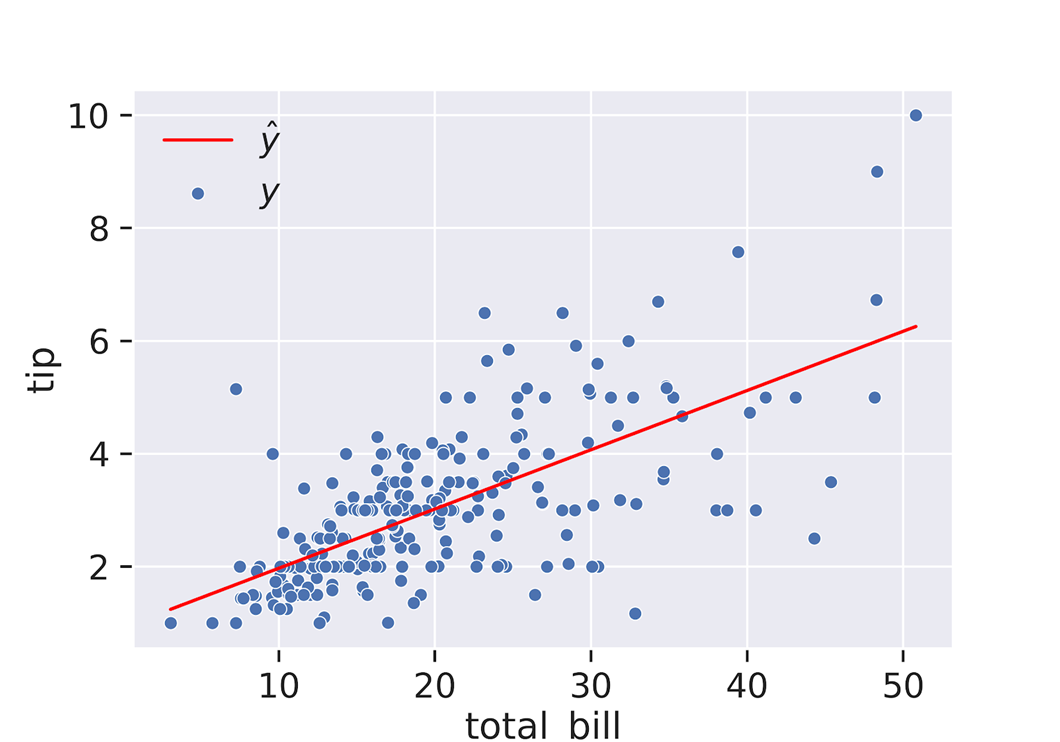
\includegraphics[scale=.4]{Bild16}
	        \end{column}
	    \end{columns}
	    
	\end{frame}
	
	
	
	
	\begin{frame}{Approach \#1: Closed Form Solution}
	    Since this is just a linear model, we can simply apply the normal equation.
	    \begin{equation*}
	        \Vec{\hat{y}} = f_{\Vec{\hat{\theta}}}(\mathbb{X}) = \mathbb{X}\Vec{\hat{\theta}}
	        \hspace{3cm} \Vec{\hat{\theta}} = (\mathbb{X}^T\mathbb{X})^{-1}\mathbb{X}^T\Vec{y}
	    \end{equation*}
	    
	    \begin{columns}
            \begin{column}{.5\textwidth}
                    \begin{equation*}
                        \mathbb{X} = \left[\begin{array}{cc}
	                                 1 & 16.99 \\
	                                 1 & 10.34 \\
	                                 1 & 21.01 \\
	                                 1 & 23.68 \\
	                                 \vdots & \vdots
	                        \end{array}\right] \hspace{.5cm} \Vec{y} = \left[\begin{array}{c}
	                             1.01  \\
	                             1.66  \\
	                             3.50  \\
	                             3.31  \\
	                             \vdots
	                        \end{array}\right]
                    \end{equation*}
            \end{column}
            
            
            \begin{column}{.5\textwidth}
                    \vspace{.5cm}\\
                    For reasons we won’t discuss, when calculating the closed form equation above, it’s generally better to use np.linalg.solve instead of np.linalg.inv.
            \end{column}
	    \end{columns}
	\end{frame}
	
	
	\begin{frame}{Approach \#2: Brute Force / Plotting}
	    As before, we could just plot the 2D loss surface and find the minimum that way (plot is easy to understand in the notebook). \\
	    \centering
	    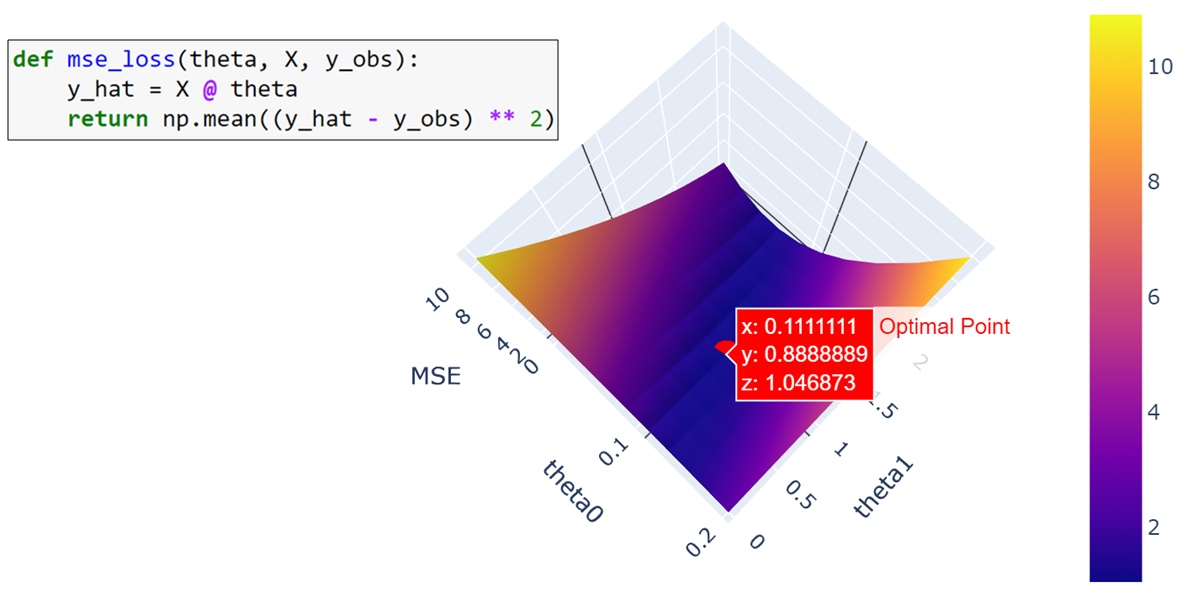
\includegraphics[scale=.35]{Bild17}
	\end{frame}
	
	
	\begin{frame}{Approach \#3: Gradient Descent}
	    Another approach is to pick a starting point on our loss surface and follow the slope to the bottom.\\
	    \begin{itemize}
	        \item On a 2D surface, the best way to go down is described by a 2D vector.
	    \end{itemize}
	    \centering
	    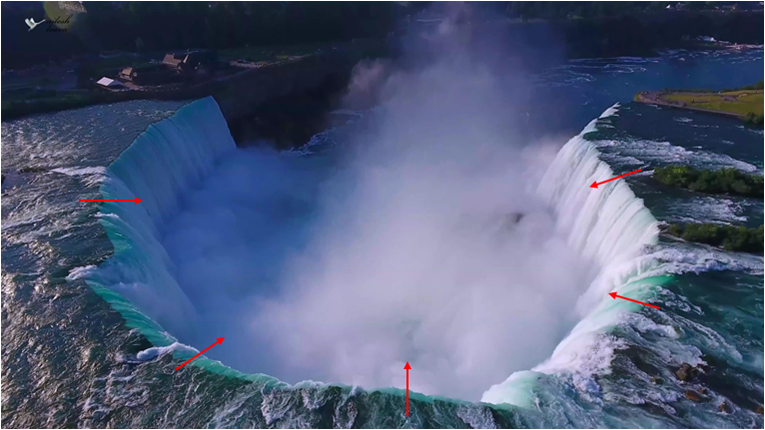
\includegraphics[scale=.45]{Bild18}
	\end{frame}
	
	
	\begin{frame}{Approach \#3: Gradient Descent}
	    On a 2D surface, the best way to go down is described by a 2D vector.\\
	    \centering
	    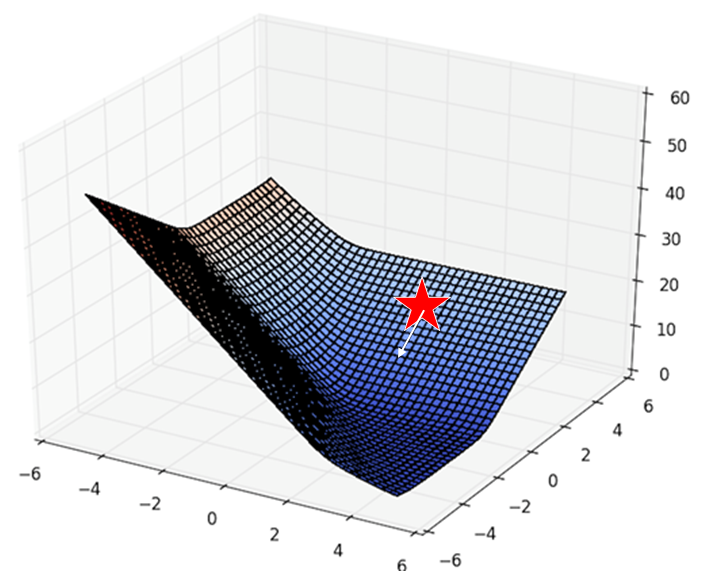
\includegraphics[scale=.4]{Bild19}
	\end{frame}
	
	\begin{frame}{Approach \#3: Gradient Descent}
	    On a 2D surface, the best way to go down is described by a 2D vector.\\
	    \centering
	    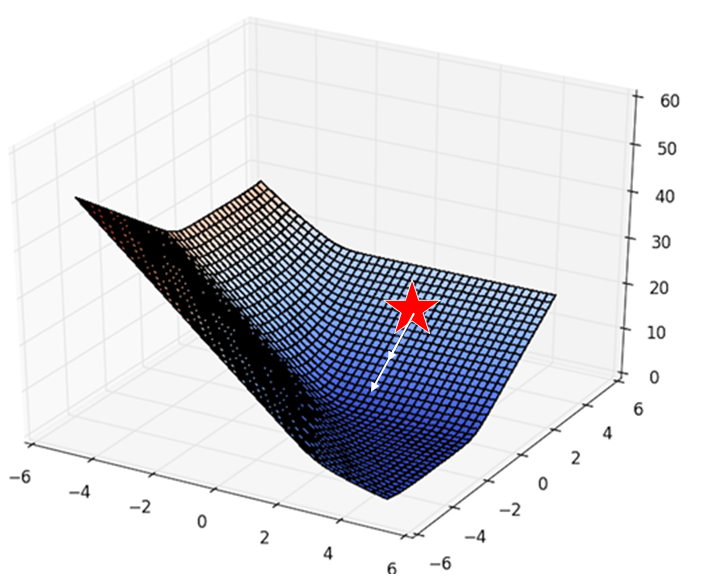
\includegraphics[scale=.4]{Bild20}
	\end{frame}
	
	\begin{frame}{Approach \#3: Gradient Descent}
	    On a 2D surface, the best way to go down is described by a 2D vector.\\
	    \centering
	    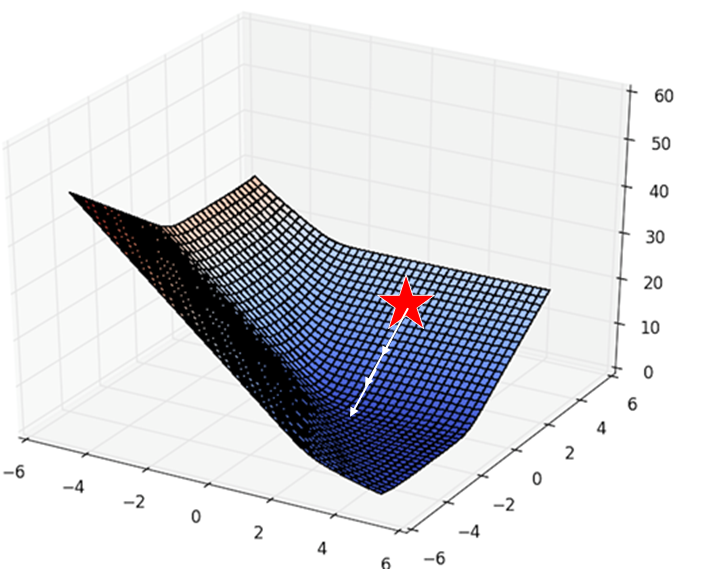
\includegraphics[scale=.4]{Bild21}
	\end{frame}
	
	
	\begin{frame}{Approach \#3: Gradient Descent}
	    On a 2D surface, the best way to go down is described by a 2D vector.\\
	    \centering
	    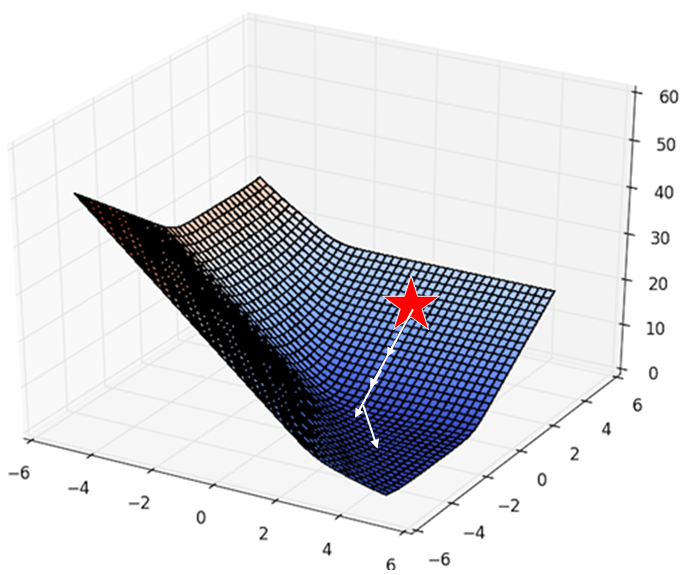
\includegraphics[scale=.4]{Bild22}
	\end{frame}
	
	
	\begin{frame}{Example: Gradient of a 2D Function}
	    Consider the 2D function: $f(\theta_0, \theta_1) = 8\theta_0^2 + 3\theta_0\theta_1$\\
	    \bigskip
	    For a function of 2 variables,     $f(\theta_0, \theta_1)$             we define the gradient           $\nabla_{\Vec{\theta}}f = \frac{\partial f}{\partial\theta_0}\Vec{i} + \frac{\partial f}{\partial\theta_1}\Vec{j} $                         , where  $\Vec{i}$   and  $\Vec{j}$   are the unit vectors in the $\theta_0$ and $\theta_1$ directions.\\
	    
	    \begin{columns}
	        \begin{column}{.5\textwidth}
	            \begin{align*}
	                &\frac{\partial f}{\partial \theta_0} = 16\theta_0 + 3\theta_1\\
	                &\frac{\partial f}{\partial \theta_1} = 3\theta_0
	            \end{align*}
	                
	        \end{column}
	        
	        
	        \begin{column}{.5\textwidth}
	                \\
	                \vspace{.7cm}
	                \begin{equation*}
	                    \nabla_{\Vec{\theta}}f = (16\theta_0 + 3\theta_1)\Vec{i} + 3\theta_0\Vec{j}
	                \end{equation*}
	        \end{column}
	    \end{columns}
	\end{frame}
	
	
	\begin{frame}{Approach \#3: Gradient Descent}
	    On a 2D surface, the best way to go down is described by a 2D vector.\\
	    \centering
	    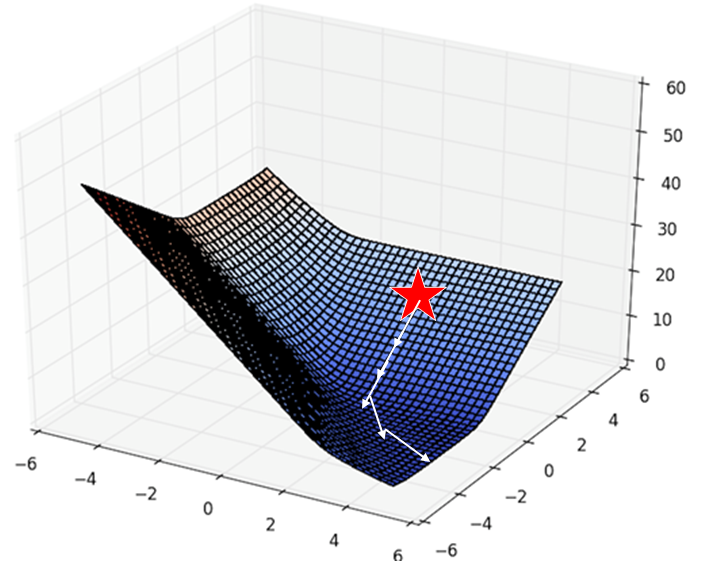
\includegraphics[scale=.4]{Bild23}
	\end{frame}
	
	
	\begin{frame}[c]{Example: Gradient of a 2D Function in Column Vector Notation}
	    Consider the 2D function:
	    \begin{equation*}
	        f(\theta_0, \theta_1) = 8\theta^2_0 + 3\theta_0\theta_1
	    \end{equation*}
	    Gradients are also often written in column vector notation.
	    \begin{equation*}
	        \nabla_{\Vec{\theta}}f(\Vec{\theta}) = \left[\begin{array}{c}
	             16\theta_0 + 3\theta_1  \\
	             3\theta_0
	        \end{array}\right]
	    \end{equation*}
	\end{frame}
	
	
	\begin{frame}[c]{Example: Gradient of a Function in Column Vector Notation}
	    For a generic function of p + 1 variables.
	    \begin{equation*}
	        \nabla_{\Vec{\theta}}f(\Vec{\theta}) = \left[\begin{array}{c}
	             \frac{\partial}{\partial\theta_0}(f)  \\
	              \frac{\partial}{\partial\theta_1}(f) \\
	              \vdots\\
	               \frac{\partial}{\partial\theta_p}(f)
	        \end{array}\right]
	    \end{equation*}
	\end{frame}
	
	
	
	\begin{frame}[c]{How to Interpret Gradients}
	    \begin{itemize}
	        \item You should read these gradients as:
	        \begin{itemize}
	            \item If I nudge the 1st model weight, what happens to loss?
	            \item If I nudge the 2nd, what happens to loss?
	            \item Etc.
	        \end{itemize}
	    \end{itemize}
	    \bigskip
	    This is similar to what you were doing when playing the loss game.
	\end{frame}
	
	
	\begin{frame}{Batch Gradient Descent}
	    \begin{itemize}
	        \item Gradient descent algorithm: nudge $\theta$ in negative gradient direction until $\theta$ converges.
	        \item Batch gradient descent update rule:
	    \end{itemize}
	    \vspace{2cm}
	    \begin{equation*}
	        \Vec{\theta}^{(t+1)} = \Vec{\theta}^{(t)} - \alpha \nabla_{\Vec{\theta}}L(\Vec{\theta}, \mathbb{X}, \Vec{y})
	    \end{equation*}
	    \vspace{-2cm}
	    
	    
	    \vspace{.7cm}
	    \hspace{2cm} 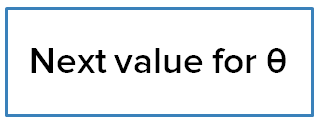
\includegraphics[scale=.3]{Bild24}\\
	    \vspace{-.7cm}
	    
	    \vspace{0.7cm}
	    \hspace{6.3cm} 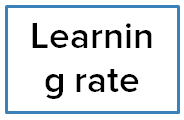
\includegraphics[scale=.3]{Bild25}\\
	    \vspace{-0.7cm}
	    
	    \vspace{-1.3cm}
	    \hspace{10.3cm} 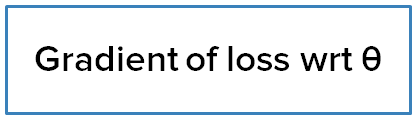
\includegraphics[scale=.3]{Bild26}\\
	    \vspace{1.3cm}
	    
	    

	    $\theta$: Model weights \hspace{2cm} L: loss function\\
	    $\alpha$: Learning rate, usually a small constant\\
	    $\gamma$: True values from the training data 
	\end{frame}
	
	
	
	\begin{frame}[c]{Gradient Descent Algorithm}
	    \begin{itemize}
	        \item Initialize model weights to all zero
	        \begin{itemize}
	            \item Also common: initialize using small random numbers
	        \end{itemize}
	        \item Update model weights using update rule:
	    \end{itemize}
	    
	    \begin{equation*}
	        \Vec{\theta}^{(t+1)} = \Vec{\theta}^{(t)} - \alpha \nabla_{\Vec{\theta}}L(\Vec{\theta}, \mathbb{X}, \Vec{y})
	    \end{equation*}
	    
	    \begin{itemize}
	        \item Repeat until model weights don’t change (convergence).
	        \begin{itemize}
	            \item At this point, we have $\hat{\theta}$ , our minimizing model weights
	        \end{itemize}
	    \end{itemize}
	\end{frame}
	
	
	\begin{frame}{The Gradient Descent Algorithm}
	    \hspace{4cm}\fbox{\parbox{.4\textwidth}{$\theta^{(0)} \leftarrow$ initial vector (random, zeros …)\\
	    For $\tau$ from 0 to convergence:\\
	    \begin{equation*}
	         \Vec{\theta}^{(t+1)} = \Vec{\theta}^{(t)} - \alpha \nabla_{\Vec{\theta}}L(\Vec{\theta}, \mathbb{X}, \Vec{y})
	    \end{equation*}}}
	    \begin{itemize}
	        \item $\alpha$ is the learning rate
	        \item Converges when gradient is $\approx$ 0 (or we run out of patience)
	    \end{itemize}
	\end{frame}
	
	
	\begin{frame}[c]{You Try:}
	    Derive the gradient descent rule for a linear model with two model weights and MSE loss. 
	    \begin{itemize}
	        \item Below we’ll consider just one observation (i.e. one row of our design matrix).
	    \end{itemize}
	    \begin{align*}
	        &f_{\Vec{\theta}}(\Vec{x}) = \Vec{x}^T\Vec{\theta} = \theta_0x_0 + \theta_1x_1\\
	        & \mathcal{L}(\Vec{\theta}, \Vec{x}, y_i) = (y_i \theta_0x_0 - \theta_1x_1)^2
	    \end{align*}
	    \begin{equation*}
	        \nabla_\theta \mathcal{L}(\Vec{\theta}, \Vec{x}, y_i) = ?
	    \end{equation*}
	    
	    \vspace{-2.5cm}
	    \hspace{10cm} 
\includegraphics[scale=.3]{Bild27}
	    \vspace{2.5cm}
	\end{frame}
	
	
	
	\begin{frame}[c]{You Try:}
	    \begin{equation*}
	        \mathcal{L}(\Vec{\theta}, \Vec{x}, y_i) = (y_i - \theta_0x_0 - \theta_1x_1)^2
	    \end{equation*}
	    \begin{align*}
	        &\frac{\partial}{\partial\theta_0}\mathcal{L}(\Vec{\theta}, \Vec{x}, y_i) = 2(y_i - \theta_0x_0 - \theta_1x_1)(-x_0)\\
	        &\frac{\partial}{\partial\theta_1}\mathcal{L}(\Vec{\theta}, \Vec{x}, y_i) = 2(y_i - \theta_0x_0 - \theta_1x_1)(-x_1)
	    \end{align*}
	    
	    \hspace{3.3cm}\fcolorbox{blue}{white}{\parbox{.55\textwidth}{The gradient for the entire dataset is the average of the gradients for each point, so we can run GD as-is.}}
	    \begin{equation*}
	        \nabla_\theta \mathcal{L}(\Vec{\theta}, \Vec{x}, y_i) = \left[\begin{array}{c}
	             -2(y_i - \theta_0x_0 - \theta_1x_1)(x_0) \\
                 -2(y_i - \theta_0x_0 - \theta_1x_1)(x_1)
	        \end{array}\right]
	    \end{equation*}
	\end{frame}
	
	
	
	\begin{frame}[c]{You Try:}
	    \begin{equation*}
	        \mathcal{L}(\Vec{\theta}, \Vec{x}, y_i) = (y_i - \theta_0x_0 - \theta_1x_1)^2
	    \end{equation*}
	    \begin{equation*}
	        \nabla_\theta \mathcal{L}(\Vec{\theta}, \Vec{x}, y_i) = \left[\begin{array}{c}
	             -2(y_i - \theta_0x_0 - \theta_1x_1)(x_0) \\
                 -2(y_i - \theta_0x_0 - \theta_1x_1)(x_1)
	        \end{array}\right]
	    \end{equation*}
	    
\includegraphics[scale=.4]{Bild28}
	\end{frame}
\end{document}